% BTVN_B8_2.tex — TDMXX23, phuong phap toa do hoa trong khong gian.
% Theo phong cach BTVN_B6.tex; hinh TikZ, khong can tep anh ngoai.
\documentclass[12pt,a4paper]{article}
\usepackage[left=15mm,right=15mm,top=14mm,bottom=18mm,footskip=9mm]{geometry}
\usepackage{iftex}
\ifPDFTeX
  \usepackage[T5]{fontenc}\usepackage[utf8]{inputenc}\usepackage{mathptmx}
\else
  \usepackage{fontspec}
  \IfFontExistsTF{Times New Roman}{\setmainfont{Times New Roman}}{%
    \IfFontExistsTF{Liberation Serif}{\setmainfont{Liberation Serif}}{\setmainfont{Latin Modern Roman}}}
\fi
\usepackage{amsmath,amssymb,fix-cm}
\usepackage{tikz}
\usetikzlibrary{arrows.meta}
\usepackage{tcolorbox,tabularx,fancyhdr,lastpage,needspace}
\definecolor{sectionpurple}{RGB}{155,42,143}
\definecolor{notebackground}{RGB}{229,240,245}
\definecolor{noteborder}{RGB}{255,55,55}
\definecolor{grblue}{RGB}{37,77,194}
\setlength{\parindent}{0pt}
\setlength{\parskip}{0pt}
\setlength{\headheight}{15pt}
\pagestyle{fancy}\fancyhf{}
\renewcommand{\headrulewidth}{0pt}\renewcommand{\footrulewidth}{0.4pt}
\fancyfoot[L]{\fontsize{8.5}{10}\selectfont Biên soạn: \textbf{Nguyễn Anh Dũng}}
\fancyfoot[R]{\fontsize{8.5}{10}\selectfont Trang \thepage/\pageref{LastPage} -- BTVN B8-2}
\newtcolorbox{notebox}{colback=notebackground,colframe=noteborder,
 boxrule=.65pt,arc=1.5pt,left=5pt,right=5pt,top=2pt,bottom=2pt,
 before skip=0pt,after skip=0pt}
\newcommand{\question}[2][TDM31]{%
  \par\noindent\textbf{\textcolor{sectionpurple}{Câu #2:} \textcolor{noteborder}{[#1]}}\enspace}
\newcommand{\answerlabel}[1]{\textbf{\textcolor{sectionpurple}{#1.}}}
\newcommand{\fourchoices}[4]{%
 \par\nobreak\vspace{1pt}\begin{tabular*}{\linewidth}{@{}l@{\extracolsep{\fill}}lll@{}}
 \answerlabel{A} #1 & \answerlabel{B} #2 & \answerlabel{C} #3 & \answerlabel{D} #4
 \end{tabular*}\par}
\newcommand{\twochoices}[4]{%
 \par\nobreak\vspace{1pt}\begin{tabularx}{\linewidth}{@{}>{\raggedright\arraybackslash}X>{\raggedright\arraybackslash}X@{}}
 \answerlabel{A} #1 & \answerlabel{B} #2 \\[1pt]
 \answerlabel{C} #3 & \answerlabel{D} #4
 \end{tabularx}\par}
\newcommand{\tfbox}[4]{%
\begin{notebox}\renewcommand{\arraystretch}{1.17}\setlength{\tabcolsep}{4pt}
\begin{tabularx}{\linewidth}{|>{\bfseries\color{sectionpurple}}c|>{\raggedright\arraybackslash}X|c|c|}
\hline\multicolumn{2}{|c|}{\textbf{\textcolor{sectionpurple}{Mệnh đề}}}&
\textbf{\textcolor{sectionpurple}{Đ}}&\textbf{\textcolor{sectionpurple}{S}}\\\hline
 a & #1 & $\bigcirc$ & $\bigcirc$ \\ \hline
 b & #2 & $\bigcirc$ & $\bigcirc$ \\ \hline
 c & #3 & $\bigcirc$ & $\bigcirc$ \\ \hline
 d & #4 & $\bigcirc$ & $\bigcirc$ \\ \hline
\end{tabularx}\end{notebox}}
\newcommand{\shortanswer}{%
 \par\nobreak\hfill
\begin{tikzpicture}[baseline=-.7ex]
 \node[draw=noteborder,fill=notebackground,line width=.6pt,rounded corners=1pt,
 minimum width=23mm,minimum height=5mm,inner sep=0pt] {};
 \end{tikzpicture}\par}
\newcommand{\examtitle}[2]{%
 \par\begin{center}\textbf{ĐỀ #1}\\[-1pt]\textbf{#2}\\[-1pt]
 {\fontsize{10.5}{12}\selectfont\itshape Form đề chuẩn bám sát BGD2026 -- Thời gian làm bài \textbf{90 phút}}\end{center}\vspace{-7pt}}
\newcommand{\partone}[1]{\par\textbf{Phần I. Câu trắc nghiệm nhiều phương án lựa chọn.} Thí sinh trả lời từ câu 1 đến câu #1. Mỗi câu chỉ chọn một phương án.\par}
\newcommand{\parttwo}[2]{\par\addvspace{2pt}\textbf{Phần II. Câu trắc nghiệm đúng sai.} Thí sinh trả lời từ câu #1 đến câu #2, trong mỗi ý a), b), c), d) chọn đúng hoặc sai.\par}
\newcommand{\partthree}[2]{\par\addvspace{2pt}\textbf{Phần III. Câu trắc nghiệm trả lời ngắn.} Thí sinh trả lời từ câu #1 đến câu #2.\par}
\newcommand{\finishExam}{\par\vspace{3pt}{\centering\textbf{\textcolor{sectionpurple}{--- Hết ---}}\par}}
% Hinh lap phuong va so do can cau duoc ve bang TikZ theo PDF (TDMXX20).
% Hinh TikZ doc lap, khong can tai tep hinh ben ngoai.
\newcommand{\figbox}[1]{%
\begin{notebox}\centering
\begin{tikzpicture}[x=.43cm,y=.43cm,>=Stealth,every node/.style={font=\fontsize{10}{11}\selectfont}]
 #1
\end{tikzpicture}\end{notebox}}
\newcommand{\axes}[4]{%
 \draw[thin,-{Stealth[length=4pt]}] (#1,0)--(#2,0) node[below] {$x$};
 \draw[thin,-{Stealth[length=4pt]}] (0,#3)--(0,#4) node[right] {$y$};
 \node[below left] at (0,0) {$O$};}
\newcommand{\dotat}[2]{\fill (#1,#2) circle (1.3pt);}
\newcommand{\vguide}[2]{\draw[thin,densely dashed] (#1,0)--(#1,#2);\dotat{#1}{0}\dotat{#1}{#2}}

\newcommand{\cubefig}{%
\begin{notebox}\centering
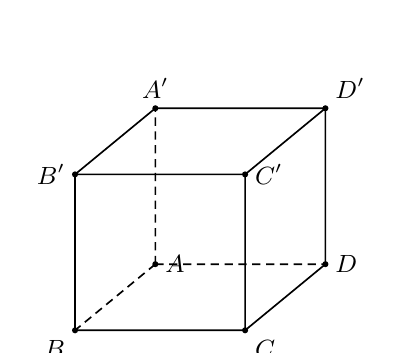
\begin{tikzpicture}[x=.60cm,y=.60cm,line width=.6pt,every node/.style={font=\small}]
 \coordinate (A) at (1.7,1.4); \coordinate (B) at (0,0);
 \coordinate (C) at (3.6,0); \coordinate (D) at (5.3,1.4);
 \coordinate (Ap) at (1.7,4.7); \coordinate (Bp) at (0,3.3);
 \coordinate (Cp) at (3.6,3.3); \coordinate (Dp) at (5.3,4.7);
 \draw[densely dashed] (A)--(B) (A)--(D) (A)--(Ap);
 \draw (B)--(C)--(D)--(Dp)--(Ap)--(Bp)--(B)
       (Bp)--(Cp)--(Dp) (Cp)--(C);
 \foreach \p in {A,B,C,D,Ap,Bp,Cp,Dp}{\fill (\p) circle (1.1pt);}
 \node[right] at (A) {$A$}; \node[below left] at (B) {$B$};
 \node[below right] at (C) {$C$}; \node[right] at (D) {$D$};
 \node[above] at (Ap) {$A'$}; \node[left] at (Bp) {$B'$};
 \node[right] at (Cp) {$C'$}; \node[above right] at (Dp) {$D'$};
\end{tikzpicture}\end{notebox}}
\newcommand{\cranefig}{%
\begin{notebox}\centering
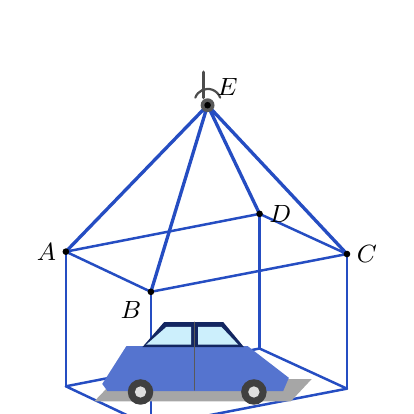
\begin{tikzpicture}[x=.60cm,y=.60cm,line join=round,line cap=round,every node/.style={font=\small}]
 \coordinate (E) at (0,6.15);
 \coordinate (A) at (-3,3.05); \coordinate (B) at (-1.20,2.20);
 \coordinate (C) at (2.95,3.00); \coordinate (D) at (1.10,3.85);
 \coordinate (Ab) at (-3,.20); \coordinate (Bb) at (-1.20,-.65);
 \coordinate (Cb) at (2.95,.15); \coordinate (Db) at (1.10,1.00);
 \draw[line width=1.2pt,grblue] (E)--(A) (E)--(B) (E)--(C) (E)--(D);
 \draw[grblue,line width=.9pt] (A)--(B)--(C)--(D)--cycle;
 \draw[grblue,line width=.9pt] (A)--(Ab) (B)--(Bb) (C)--(Cb) (D)--(Db);
 \draw[grblue,line width=.9pt] (Ab)--(Bb)--(Cb)--(Db)--cycle;
 \draw[very thick,gray!60!black] (-.08,6.85)--(-.08,6.31);
 \fill[gray!70!black] (E) circle (2.5pt);
 \draw[thick,gray!60!black] (-.26,6.31) arc[start angle=160,end angle=20,radius=.28];
 \fill[black!35] (-2.40,-.12)--(1.76,-.12)--(2.20,.35)--(-1.95,.35)--cycle;
 \fill[grblue!78] (-2.23,.25)--(-1.72,1.05)--(.85,1.05)--(1.72,.38)--(1.60,.10)--(-2.12,.10)--cycle;
 \fill[grblue!50!black] (-1.38,1.03)--(-.92,1.56)--(.33,1.56)--(.77,1.03)--cycle;
 \fill[cyan!20] (-1.30,1.08)--(-.87,1.46)--(-.35,1.46)--(-.35,1.08)--cycle;
 \fill[cyan!20] (-.20,1.08)--(-.20,1.46)--(.29,1.46)--(.65,1.08)--cycle;
 \draw[black!65,thin] (-.27,.12)--(-.27,1.56);
 \fill[black!75] (-1.42,.08) circle (.27) (.98,.08) circle (.27);
 \fill[gray!25] (-1.42,.08) circle (.12) (.98,.08) circle (.12);
 \foreach \p/\where in {E/above right,A/left,B/below left,C/right,D/right}
    {\fill (\p) circle (1.2pt);\node[\where] at (\p) {$\p$};}
\end{tikzpicture}\end{notebox}}


% Hinh dung TikZ, khong phu thuoc tep anh ngoai.
\newcommand{\pyramidcoordfig}{%
\begin{notebox}\centering
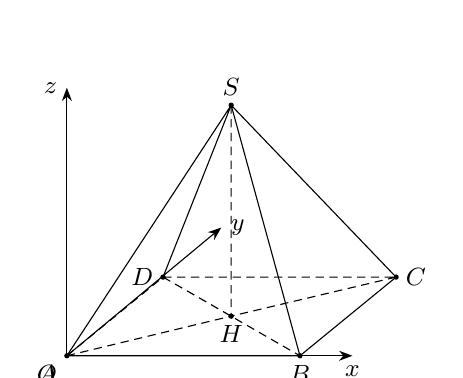
\begin{tikzpicture}[scale=.74,>=Stealth, every node/.style={font=\small}]
\coordinate (A) at (0,0); \coordinate (B) at (4,0);
\coordinate (D) at (1.65,1.35); \coordinate (C) at (5.65,1.35);
\coordinate (H) at (2.82,.68); \coordinate (S) at (2.82,4.3);
\draw[thin,-{Stealth}] (A)--(4.9,0) node[below] {$x$};
\draw[thin,-{Stealth}] (A)--(0,4.6) node[left] {$z$};
\draw[thin,-{Stealth}] (A)--(2.65,2.2) node[right] {$y$};
\draw[densely dashed] (A)--(D)--(C) (D)--(B) (A)--(H) (D)--(H) (C)--(H) (S)--(H);
\draw (A)--(B)--(C) (S)--(A) (S)--(B) (S)--(C) (S)--(D);
\foreach \p/\pos in {A/below left,B/below,C/right,D/left,H/below,S/above}
{\fill (\p) circle (1.3pt); \node[\pos] at (\p) {$\p$};}
\node[below left] at (A) {$O$};
\end{tikzpicture}\end{notebox}}
\newcommand{\roomcoordfig}{%
\begin{notebox}\centering
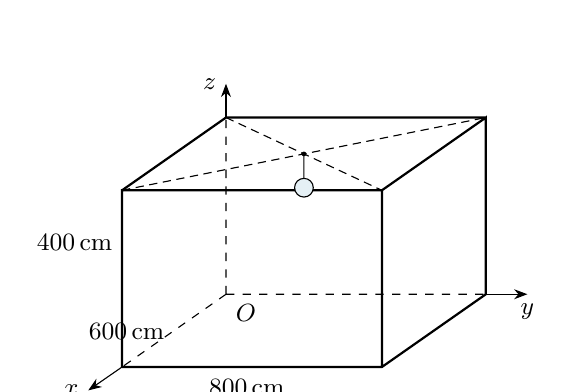
\begin{tikzpicture}[scale=.66,>=Stealth,every node/.style={font=\small}]
\coordinate (O) at (0,0); \coordinate (X) at (-2,-1.4);
\coordinate (Y) at (5,0); \coordinate (Z) at (0,3.4);
\coordinate (XY) at (3,-1.4); \coordinate (XZ) at (-2,2);
\coordinate (YZ) at (5,3.4); \coordinate (XYZ) at (3,2);
\draw[dashed] (O)--(X) (O)--(Y) (O)--(Z);
\draw[thick] (X)--(XY)--(Y)--(YZ)--(XYZ)--(XZ)--(X)
 (XZ)--(Z)--(YZ) (XYZ)--(XY);
\draw[densely dashed] (Z)--(XYZ) (XZ)--(YZ);
\coordinate (P) at (1.5,2.7);
\draw[thin] (P)--(1.5,2.18);
\draw[fill=notebackground] (1.5,2.05) circle (.18);
\fill (P) circle (1.3pt);
\node[below right] at (O) {$O$};
\draw[-{Stealth}] (X)--(-2.65,-1.85) node[left] {$x$};
\draw[-{Stealth}] (Y)--(5.8,0) node[below] {$y$};
\draw[-{Stealth}] (Z)--(0,4.05) node[left] {$z$};
\node[below] at (.4,-1.45) {$800\,\mathrm{cm}$};
\node[left] at (-1,-.72) {$600\,\mathrm{cm}$};
\node[left] at (-2,1.0) {$400\,\mathrm{cm}$};
\end{tikzpicture}\end{notebox}}
\newcommand{\cubecoordsfig}{%
\begin{notebox}\centering
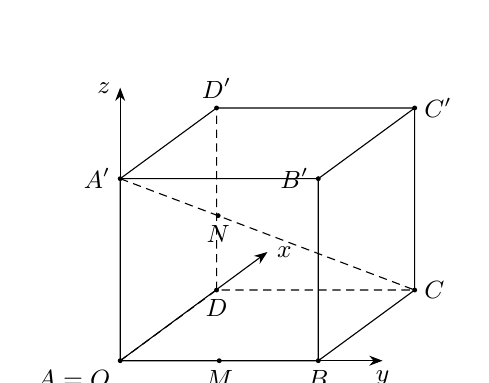
\begin{tikzpicture}[scale=.68,>=Stealth,every node/.style={font=\small}]
\coordinate (A) at (0,0); \coordinate (B) at (3.7,0);
\coordinate (D) at (1.8,1.32); \coordinate (C) at (5.5,1.32);
\coordinate (Ap) at (0,3.4); \coordinate (Bp) at (3.7,3.4);
\coordinate (Dp) at (1.8,4.72); \coordinate (Cp) at (5.5,4.72);
\coordinate (M) at (1.85,0); \coordinate (N) at (1.83,2.71);
\draw[densely dashed] (A)--(D)--(C) (D)--(Dp) (Ap)--(C);
\draw (A)--(B)--(C)--(Cp)--(Dp)--(Ap)--(A)
 (Ap)--(Bp)--(Cp) (Bp)--(B);
\draw[-{Stealth}] (A)--(4.9,0) node[below] {$y$};
\draw[-{Stealth}] (A)--(2.75,2.03) node[right] {$x$};
\draw[-{Stealth}] (A)--(0,5.1) node[left] {$z$};
\foreach \p/\pos/\lab in {A/below left/{A=O},B/below/B,C/right/C,D/below/D,Ap/left/{A'},Bp/left/{B'},Cp/right/{C'},Dp/above/{D'},M/below/M,N/below/N}
{\fill (\p) circle (1.3pt); \node[\pos] at (\p) {$\lab$};}
\end{tikzpicture}\end{notebox}}
\newcommand{\ballooncoordfig}{%
\begin{notebox}\centering
\begin{tikzpicture}[scale=.75,>=Stealth,every node/.style={font=\small}]
\draw[->] (0,0)--(2.5,-1.2) node[below] {Nam ($x$)};
\draw[->] (0,0)--(4,0) node[right] {Đông ($y$)};
\draw[->] (0,0)--(0,3.1) node[left] {$z$};
\node[below left] at (0,0) {$O$};
\draw[densely dashed] (3.3,.7)--(3.3,-.1);
\draw[densely dashed] (-1.0,2.2)--(-1,-.2);
\foreach \x/\y/\c in {3.3/.9/cyan,-1/2.4/orange}{
\fill[\c!30,draw=grblue] (\x,\y) ellipse (.37 and .47);
\draw (\x-.17,\y-.39)--(\x-.1,\y-.66)--(\x+.1,\y-.66)--(\x+.17,\y-.39);
\fill[brown!50] (\x-.12,\y-.72) rectangle (\x+.12,\y-.61);}
\node[right] at (3.65,1.2) {Bóng 1};
\node[left] at (-1.35,2.5) {Bóng 2};
\end{tikzpicture}\end{notebox}}
\newcommand{\seacoordfig}{%
\begin{notebox}\centering
\begin{tikzpicture}[scale=.78,>=Stealth,every node/.style={font=\small}]
\fill[cyan!10] (-3,-.7) rectangle (5,0);
\draw[cyan!60] (-3,0)--(5,0);
\fill[gray!65] (-.65,-.2) rectangle (.6,.55);
\draw[very thick,gray!70!black] (-.1,.55)--(-.1,1.65);
\draw[->,red] (0,0)--(3,1.4) node[right] {$y$ (Nam)};
\draw[->,red] (0,0)--(-2.4,0) node[left] {$x$ (Tây)};
\draw[->,red] (0,0)--(0,2.7) node[above] {$z$};
\draw[densely dashed] (0,0)--(2,-1.8);
\draw[fill=black!60,rounded corners=3pt] (1.5,-1.85) rectangle (2.5,-1.63);
\node[right] at (2.5,-1.7) {Tàu ngầm};
\node[below left] at (0,0) {$O$};
\end{tikzpicture}\end{notebox}}

\begin{document}
\fontsize{11.5}{14}\selectfont
\examtitle{TDMXX23}{PHƯƠNG PHÁP TỌA ĐỘ HÓA TRONG KHÔNG GIAN}
\partone{12}
\noindent\textbf{Sử dụng đề bài để hoàn thành câu 1, câu 2, câu 3:}
Cho hình lập phương $ABCD.A'B'C'D'$ có cạnh bằng $1$. Chọn hệ trục tọa độ $Oxyz$ sao cho điểm $A$ trùng với gốc $O$, trục $Ox$ hướng theo vectơ $\overrightarrow{AB}$, trục $Oy$ hướng theo vectơ $\overrightarrow{AD}$, trục $Oz$ hướng theo vectơ $\overrightarrow{AA'}$.
\question[TDM21]{1} Tọa độ của điểm $C'$ là
\fourchoices{$(1;1;1)$.}{$(1;1;0)$.}{$(1;1;-1)$.}{$(0;0;1)$.}
\question[TDM21]{2} Tọa độ của vectơ $\overrightarrow{BD'}$ là
\fourchoices{$(1;1;-1)$.}{$(-1;0;1)$.}{$(0;2;\sqrt3)$.}{$(-1;1;1)$.}
\question[TDM21]{3} Tọa độ của vectơ $\overrightarrow{A'D}+\overrightarrow{BC'}$ là
\fourchoices{$(0;2;2)$.}{$(2;0;2)$.}{$(0;2;0)$.}{$(2;0;0)$.}

% Ban goc co them mot cau duoc danh so 5 nam truoc cum cau 4-6.
% Giu nguyen de tranh bo sot du lieu; khong tu y sua so thu tu cua de nguon.
\question[TDM21]{5} Sau khi ta gắn hệ trục tọa độ $Oxyz$ vào hình lập phương $ABCD.A'B'C'D'$ thì thu được tọa độ các điểm $A(1;0;0)$, $C(0;1;0)$, $B'(0;0;1)$. Hỏi gốc tọa độ $O$ trùng với điểm nào dưới đây?
\fourchoices{$A'$.}{$D$.}{$B$.}{$C'$.}

\noindent\textbf{Sử dụng đề bài để hoàn thành câu 4, câu 5, câu 6:}
Sau khi ta gắn hệ trục tọa độ $Oxyz$ vào hình lập phương $ABCD.A'B'C'D'$ thì thu được tọa độ các điểm $A(2;0;0)$, $C(0;2;0)$, $B'(0;0;2)$.
\question[TDM21]{4} Hỏi gốc tọa độ $O$ trùng với điểm nào dưới đây?
\fourchoices{$A'$.}{$D$.}{$B$.}{$C'$.}
\question[TDM21]{5} Thể tích của hình lập phương $ABCD.A'B'C'D'$ bằng
\fourchoices{$2$.}{$8$.}{$1$.}{$6$.}
\question[TDM21]{6} Tọa độ vectơ $\left[\overrightarrow{AC},\overrightarrow{B'D}\right]$ bằng
\fourchoices{$(-4;-4;-8)$.}{$(4;-4;8)$.}{$(-2;-2;-4)$.}{$(1;1;2)$.}

\noindent\textbf{Sử dụng đề bài để hoàn thành câu 7, câu 8, câu 9:}
Sau khi ta gắn hệ trục tọa độ $Oxyz$ vào hình chóp đều $S.ABCD$ như hình vẽ, ta thu được tọa độ các điểm $B(4;0;0)$, $S(a;b;3)$.
\pyramidcoordfig
\question[TDM21]{7} Giá trị của $a+b$ bằng
\fourchoices{$6$.}{$4$.}{$9$.}{$2\sqrt3$.}
\question[TDM31]{8} Tọa độ của vectơ pháp tuyến $(SAB)$ là
\fourchoices{$(0;-12;-8)$.}{$(0;12;8)$.}{$(3;0;-2)$.}{$(0;6;-4)$.}
\question[TDM31]{9} Hãy xác định \textbf{cosin} của góc giữa hai mặt phẳng $(SAB)$ và $(SAC)$ bằng
\fourchoices{$\dfrac{3}{\sqrt{26}}$.}{$\dfrac{3}{\sqrt{13}}$.}{$\dfrac34$.}{$\dfrac{1}{\sqrt3}$.}

\noindent\textbf{Sử dụng đề bài để hoàn thành câu 10, câu 11, câu 12:}
Cho một phòng khách dạng hình hộp chữ nhật kích thước $800\,\mathrm{cm}\times600\,\mathrm{cm}\times400\,\mathrm{cm}$ như hình vẽ, có treo một chiếc đèn dạng hình cầu ở chính giữa phòng. Biết dây treo đèn dài $20\,\mathrm{cm}$ và đường kính đèn bằng $30\,\mathrm{cm}$. Ta gắn hệ trục tọa độ $Oxyz$ vào như hình vẽ. Biết đơn vị độ dài trên mỗi trục là $100\,\mathrm{cm}$.
\roomcoordfig
\question[TDM21]{10} Tọa độ điểm treo đèn là
\fourchoices{$(4;3;4)$.}{$(3;4;4)$.}{$(6;8;4)$.}{$(8;6;4)$.}
\question[TDM31]{11} Tọa độ điểm thấp nhất của đèn là
\fourchoices{$(3;4;2)$.}{$(3;4;3)$.}{$(3;4;\dfrac{19}{5})$.}{$(3;4;\dfrac72)$.}
\question[TDM31]{12} Khoảng cách từ điểm thấp nhất đến một góc dưới của phòng là
\twochoices{$100\sqrt{13}\,(\mathrm{cm})$.}{$500\,(\mathrm{cm})$.}{$50\sqrt{149}\,(\mathrm{cm})$.}{$540\,(\mathrm{cm})$.}

\parttwo{13}{16}
\question[TDM32]{13} Cho hình hộp chữ nhật $ABCD.A'B'C'D'$ có $AB=2$, $AD=3$, $AA'=4$. Gắn hệ trục tọa độ $Oxyz$ vào $ABCD.A'B'C'D'$ như sau: Gốc $O$ trùng với điểm $A$, trục $Ox$ hướng theo vectơ $\overrightarrow{AD}$, trục $Oy$ hướng theo vectơ $\overrightarrow{AA'}$, trục $Oz$ hướng theo vectơ $\overrightarrow{AB}$. Gọi $M$ là trung điểm của cạnh $A'B$. Mệnh đề nào sau đây là \textbf{đúng hay sai}?
\tfbox{Tọa độ các điểm $A(0;0;0)$, $A'(0;0;4)$.}
{$M(0;2;1)$.}
{Nếu $\varphi$ là góc giữa đường thẳng $CM$ và mặt phẳng $(AB'D)$ thì $\cos\varphi=\dfrac{\sqrt3}{2}$.}
{$d\left(C,(MC'D')\right)=1$.}

\question[TDM32]{14} Cho hình chóp tứ giác đều $S.ABCD$ với cạnh $AB=2$. Ta tiến hành gắn hệ trục tọa độ $Oxyz$ vào hình chóp $S.ABCD$, với gốc $O$ là giao của $AC$ và $BD$, có tọa độ của các điểm là $S(0;0;2)$, trục $Ox$ hướng theo vectơ $\overrightarrow{CA}$, trục $Oy$ hướng theo vectơ $\overrightarrow{DB}$. Mệnh đề nào sau đây là \textbf{đúng hay sai}?
\tfbox{Trục $Oz$ hướng theo vectơ $\overrightarrow{AS}$.}
{Tọa độ của điểm $A$ là $(\sqrt2;0;0)$ và tọa độ điểm $D$ là $(0;-\sqrt2;0)$.}
{Hình chóp $S.ABCD$ có chiều cao bằng $2$ và cạnh bên bằng $\sqrt6$.}
{Gọi $\varphi$ là góc giữa hai mặt phẳng $(SAB)$ và $(SBC)$ thì $\cos\varphi=\dfrac12$.}

\question[TDM32]{15} Cho hình lập phương $ABCD.A'B'C'D'$ có cạnh bằng $1$. Gọi $M$ là trung điểm của $AB$ và $N$ là điểm nằm trên cạnh $A'C$ sao cho $NC=2NA'$. Ta gắn hệ trục tọa độ $Oxyz$ vào hình lập phương như hình vẽ.
\cubecoordsfig
Mệnh đề nào dưới đây là \textbf{đúng hay sai}?
\tfbox{Tọa độ điểm $C(1;1;0)$.}
{Tọa độ các điểm $M\left(0;\dfrac12;0\right)$, $N(0;1;1)$.}
{$MN=\dfrac{\sqrt{21}}{6}$.}
{Gọi $\varphi$ là góc giữa $MN$ và mặt phẳng $(BCD')$ thì $\cos\varphi=\dfrac{1}{\sqrt7}$.}

\question[TDM32]{16} Trong không gian $Oxyz$, cho hình chóp $S.ABC$ có đáy là tam giác vuông tại $A$, biết tọa độ các điểm $S(0;0;3)$, $B(0;4;0)$, $C(0;-2;0)$. Biết điểm $A$ có hoành độ bằng $2$, có tung độ dương và có cao độ bằng $0$. Mệnh đề nào sau đây là \textbf{đúng hay sai}?
\tfbox{Điểm $A$ thuộc mặt phẳng tọa độ $(Oxy)$.}
{$(SBC)\perp(ABC)$.}
{Tọa độ điểm $A$ là $(2;1+\sqrt3;0)$.}
{Thể tích của hình chóp $S.ABC$ bằng $6$.}

\partthree{17}{22}
\question[TDM32]{17} Cho hai chiếc khinh khí cầu bay lên từ cùng một điểm ta gọi là $O$. Ở cùng một thời điểm ta thu được vị trí chiếc thứ nhất: cách điểm $O$ $3\,\mathrm{km}$ về phía nam, $2\,\mathrm{km}$ về phía đông, cách mặt đất $0{,}7\,\mathrm{km}$; chiếc thứ hai: cách điểm $O$ $4\,\mathrm{km}$ về phía nam, $1\,\mathrm{km}$ về phía tây, cách mặt đất $0{,}5\,\mathrm{km}$. Hãy xác định khoảng cách giữa hai khinh khí cầu ở thời điểm đó theo đơn vị kilômét (làm tròn kết quả đến hàng phần trăm)?
\ballooncoordfig
\shortanswer

\question[TDM32]{18} Cho hình chóp $S.ABCD$ có đáy $ABCD$ là hình chữ nhật, cạnh bên $SA$ vuông góc với đáy $(ABCD)$ và $SA=AB=2AD$. Gọi $M$ là trung điểm của $SB$ và $N$ nằm trên cạnh $SD$ sao cho $2NS=ND$. Hãy xác định \textbf{sin} của góc tạo bởi $SC$ và mặt phẳng $(CMN)$ (làm tròn kết quả đến hàng phần trăm)?
\shortanswer

\question[TDM32]{19} Gắn hệ trục tọa độ $Oxyz$ vào không gian biển, với gốc $O$ là trung tâm của một giàn khoan trên biển, mặt phẳng $(Oxy)$ trùng với mặt biển, trục $Ox$ hướng dọc về tây, trục $Oy$ hướng dọc về nam, trục $Oz$ hướng thẳng đứng lên trên, đơn vị độ dài trên mỗi trục tọa độ là $10\,\mathrm{km}$. Ở một thời điểm radar đặt tại $O$ phát hiện được một tàu ngầm ở cách $O$ là $80{,}1\,\mathrm{km}$ và đang có hoành độ và tung độ lần lượt là $6{,}24$ và $5{,}022$. Hãy xác định độ sâu so với mặt biển của tàu ngầm đó theo đơn vị mét (làm tròn kết quả đến hàng đơn vị)?
\seacoordfig
\shortanswer

\question[TDM32]{20} Cho hình lập phương $ABCD.A'B'C'D'$ có cạnh bằng $a$. Gọi $M$ là trung điểm của $AB$ và $N$ là điểm nằm trên cạnh $A'C$ sao cho $NA'=3NC$. Hãy xác định \textbf{cosin} góc giữa hai mặt phẳng $(MA'C')$ và $(NC'D)$? (Kết quả được làm tròn và lấy hai chữ số sau dấu phẩy.)
\shortanswer

\question[TDM42]{21} Cho hình lăng trụ đứng $ABC.A'B'C'$ có đáy là tam giác vuông tại $A$ và có $AA'=AB$, $AC=a$. Gọi $M,N$ lần lượt là trung điểm của các cạnh $AB,CC'$. Biết giá trị \textbf{cosin} góc giữa hai mặt phẳng $(A'MN)$ và $(ABC)$ bằng $\dfrac25$. Biết thể tích khối lăng trụ $ABC.A'B'C'$ bằng $xa^3$. Hãy xác định giá trị của $x$? (Kết quả được làm tròn và lấy một chữ số sau dấu phẩy.)
\shortanswer

\question[TDM42]{22} Cho hình chóp $S.ABC$ có đáy là tam giác đều cạnh $4$ và cạnh bên $SA$ vuông góc với đáy. Gọi $M$ là trung điểm của $SB$ và điểm $N$ nằm trên cạnh $SC$ sao cho $\overrightarrow{NS}+2\overrightarrow{NC}=\vec0$. Biết góc tạo bởi hai mặt phẳng $(ABC)$ và $(AMN)$ là $\varphi$ và có $\cos\varphi=\dfrac1{\sqrt5}$. Hãy xác định thể tích khối chóp $S.ABC$? (Kết quả được làm tròn và lấy một chữ số sau dấu phẩy.)
\shortanswer
\finishExam

% Nguon: DE TDMXX23_DTL_PHUONG PHAP TOA DO HOA TRONG KG.pdf, 5 trang.
% Ban goc danh nham/danh trung "Cau 5" tren trang 1; van giu toan bo cau hoi.
\end{document}